%%%%%%%%%%%%%%%%%%%%%%%%%%%%%%%%%%%%%%%%%%%%%%%%%%%%%%%%%%%%%%%%%%%%%%%%
\chapter{Background}
\label{chapter:ch2-background}
%%%%%%%%%%%%%%%%%%%%%%%%%%%%%%%%%%%%%%%%%%%%%%%%%%%%%%%%%%%%%%%%%%%%%%%%
\localtableofcontents
\vspace{\marginbellowtable}


This chapter gives a short introduction on the theory of supervised learning~\cite{shalev2014understanding} and Toeplitz matrices~\cite{gray2006toeplitz}.
In the statistical learning framework, supervised learning refers to the problem of optimizing the parameters of a function in order to map an input to an output based on a series of input-output pairs.
For example, an image (input) mapped to a class (output) describing its content.
The first section describes a formal model that aims to describe such learning tasks.
In linear algebra, a Toeplitz matrix, named after Otto Toeplitz, is a matrix in which each descending diagonal, from left to right, is constant.
The second section describes the mathematical properties of Toeplitz matrices and known theorems that we use in this thesis. 


%%%%%%%%%%%%%%%%%%%%%%%%%%%%%%%%%%%%%%%%%%%%%%%%%%%%%%%%%%%%%%%%%%%%%%%%%%%%%%%
\section{Introduction on Supervised Learning}
\label{section:ch2-introduction_on_supervised_learning}
%%%%%%%%%%%%%%%%%%%%%%%%%%%%%%%%%%%%%%%%%%%%%%%%%%%%%%%%%%%%%%%%%%%%%%%%%%%%%%%

\begin{figure}[t]
  \centering
  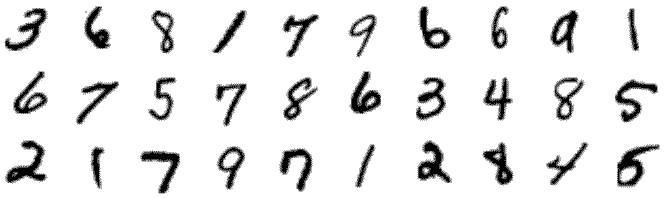
\includegraphics[width=0.85\textwidth]{figures/main/ch2-background/mnist-dataset.png}
  \caption{Images with handwritten digits in the MNIST database \cite{lecun1998gradient}}
  \label{figure:ch2-mnist-database}
\end{figure}


In \citeyear{lecun1998gradient}, \citeauthor{lecun1998gradient} had successfully learned a function capable of recognizing handwritten digits in images.
They used the MNIST database \cite{lecun1998gradient} which consists of black and white images of size $28 \times 28$ pixels (see Figure~\ref{figure:ch2-mnist-database}).
Their goal was to build a machine that takes a vector as input and produces the identity of the digit $0 \dots 9$ as the output.
This is a non-trivial problem because each image is unique and while digits can be differentiated based on their shapes and strokes, these features give poor results for an automated system. 

In the following, we will formalize the learning problem describe above with the \emph{statistical learning framework}.
First, let us define the domain space $\mathcal{X}$ which corresponds to the set of images that we wish to label.
In our example above, this domain corresponds to the set of all possible images with handwritten digits.
Let us denote the label space $\mathcal{Y}$ and a finite sequence of pairs $\mathcal{S} = \left\{ \left(\xvec^{(1)}, y^{(1)} \right) \dots \left( \xvec^{(m)}, y^{(m)} \right) \right\}$ in $\mathcal{X} \times \mathcal{Y}$. 
Such pairs \ie, labeled examples, are called \emph{training examples} and the set $\mathcal{S}$ is called the \emph{training set}.
We denote $\mathcal{D}$ the \emph{joint distribution} over $\mathcal{X} \times \mathcal{Y}$.
The main objective of the task at hand is to output a \emph{prediction rule} $h: \mathcal{X} \rightarrow \mathcal{Y}$ that maps the input $\xvec \in \mathcal{X}$ to the output $y \in \mathcal{Y}$.
This function is called the \emph{hypothesis} or the \emph{classifier}. 
Given the probability distribution $\mathcal{D}$, we aim to measure how \emph{likely} the hypothesis $h$ makes an error when labeled points are randomly drawn from the distribution $\mathcal{D}$.
Let us define the true error or \emph{risk} of the hypothesis $h$ that we which to minimize:
\begin{equation}
  R_{\mathcal{D}}(h) \triangleq \Pbb_{(\xvec, y) \sim \mathcal{D}} \left[ h(\xvec) \neq  y \right] \enspace.
  \label{equation:ch2-risk1}
\end{equation}
However, in practice, the joint probability distribution $\mathcal{D}$ is unknown; therefore, the true error is not directly available to the learner.
The learner only has access to the training data, $\mathcal{S}$, and can calculate the \emph{empirical error} \ie, the error over the training samples.
We define the \emph{empirical risk} as follows:
\begin{equation}
  R_{\mathcal{S}}(h) \triangleq \frac{\left| \left\{i \in [m]: h\left(\xvec^{(i)}\right) \neq y^{(i)} \right\}\right|}{m} \enspace.
\end{equation}
We can generalize our measure of correctness so that it can be applied to multiple learning tasks.
Let us define a \emph{loss function} from $\mathcal{Y} \times \mathcal{Y}$ to the set of nonnegative real numbers, $L: \mathcal{Y} \times \mathcal{Y} \rightarrow \Rbb_{+}$.
We can express the \emph{risk} as follows:
\begin{equation}
  R_{\mathcal{D}}(h) \triangleq \Ebb_{(\xvec, y) \sim \mathcal{D}} \left[ L\big( h(\xvec), y \big) \right] \enspace.
  \label{equation:ch2-risk2}
\end{equation}
Similarly, we express the empirical risk as follows:
\begin{equation}
  R_{\mathcal{S}}(h) \triangleq \frac{1}{m} \sum_{(\xvec, y) \sim \mathcal{S}} L\big( h(\xvec), y \big) \enspace.
\end{equation}
The loss functions used for classification problems and regression problems are as follows: 
\begin{itemize}
  \item \textbf{0-1 Loss}: $L_{0-1}\big( h(\xvec), y \big) = \mathds{1}\big[ h(\xvec) \neq y \big]$ \\
  This loss is used for classification problems, for example, when the learner have to recognizing hand-written digits in images.
  We can notice that the definitions of $R_{\mathcal{D}}$ given in Equation~\ref{equation:ch2-risk1} and Equation~\ref{equation:ch2-risk2} coincide.
  \item \textbf{Square Loss}: $L_{\text{sq}} \big( h(\xvec), y \big) = \big( h(\xvec) - y \big)^2$ \\	
  This loss is used for another common type of learning problem \ie, \emph{regression problem}, in which the label domain $\mathcal{Y}$ is the set of real numbers.
  For example, one wishes to predict the price of an apartment given its characteristics.
\end{itemize}


\noindent
The goal of the learning algorithm is to find the hypothesis $h$ that minimize the risk $R_{\mathcal{S}}$, this learning paradigm is called \emph{Empirical Risk Minimization} (ERM).
We use the ERM paradigm as a surrogate to find a hypothesis $h$ that minimize the true risk $R_\mathcal{D}$.
However, all hypothesis that minimize the empirical error does not necessarily minimize the true risk.
For example, consider the following function:
\begin{equation}
  h^*(\xvec) =
  \begin{cases}
    y^{(i)} &\quad \text{if }\exists i \in [m] \text{ s.t. } \xvec^{(i)} = \xvec \\
    0 &\quad \text{otherwise}
  \end{cases}
  \label{equation:ch2-perfect_function}
\end{equation}
Clearly, this function, for any training set, $\mathcal{S}$, will have $R_\mathcal{S}(h^*) = 0$, whereas the true risk would certainly be high.
The phenomenon, called \emph{overfitting}, happens when the classifier fits the training data ``too well'' but will likely have a high error on unseen data.
One possible solution to this phenomenon is to apply ERM with a restricted search space to prevent the learning algorithm to output a function such as $h^*$ in Equation~\ref{equation:ch2-perfect_function}.
We call this set the \emph{hypothesis class} and is denoted $\mathcal{H}$. 
Each $h \in \mathcal{H}$ is a function mapping from $\mathcal{X}$ to $\mathcal{Y}$.
We call $\mathrm{ERM}_{\mathcal{H}}$, the learned that use the $\mathrm{ERM}$ paradigm over the hypothesis class $\mathcal{H}$ and a training data $\mathcal{S}$.
Formally,
\begin{equation}
  \mathrm{ERM}_{\mathcal{H}}(\mathcal{S}) \in \argmin_{h \in \mathcal{H}} R_{\mathcal{S}}(h) \enspace.
\end{equation}
For a training sample $\mathcal{S}$, we denote $h_\mathcal{S}$, one solution of applying $\text{ERM}_\mathcal{H}$ on the set $\mathcal{S}$, if there exists multiple hypotheses with minimal error on the training sample, then minimization problem returns an arbitrary one.
In practice, the hypothesis class is chosen based on a hypothesis on the relation between the data and its label.
For example, if the relation between the data and its label is supposedly linear then the hypothesis class can be the set of all linear function.
This kind of restriction is called an \emph{inductive bias} because the learner is \emph{biased} toward a particular set of predictors.

\begin{figure}[t]
  \centering
  \begin{subfigure}[b]{0.32\textwidth}
    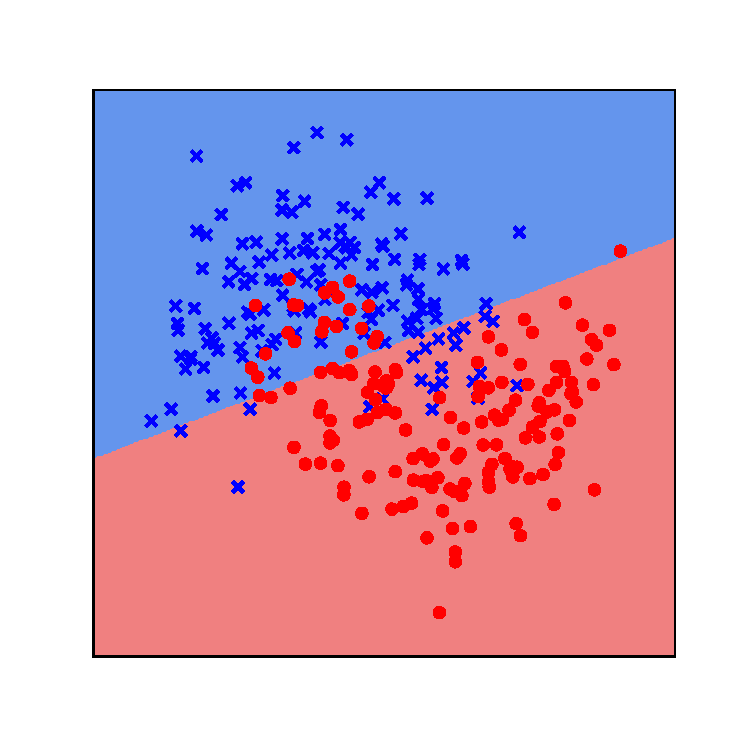
\includegraphics[width=0.98\textwidth]{figures/main/ch2-background/underfitting.pdf}
    \caption{Underfitting}
    \label{figure:ch2-fitting_points_a}
  \end{subfigure}
  \hfill
  \begin{subfigure}[b]{0.32\textwidth}
    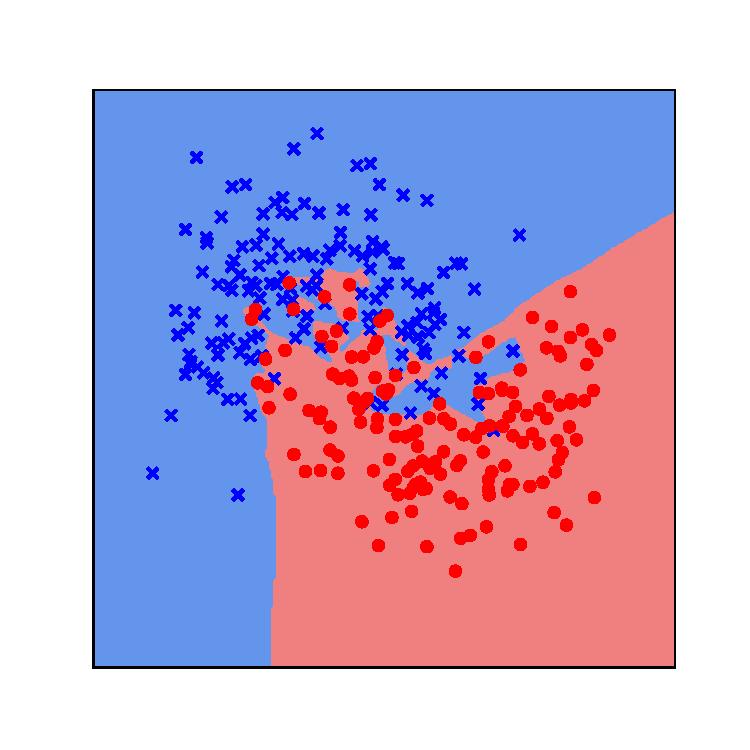
\includegraphics[width=0.98\textwidth]{figures/main/ch2-background/overfitting.pdf}
    \caption{Overfitting}
    \label{figure:ch2-fitting_points_b}
  \end{subfigure}
  \hfill
  \begin{subfigure}[b]{0.32\textwidth}
    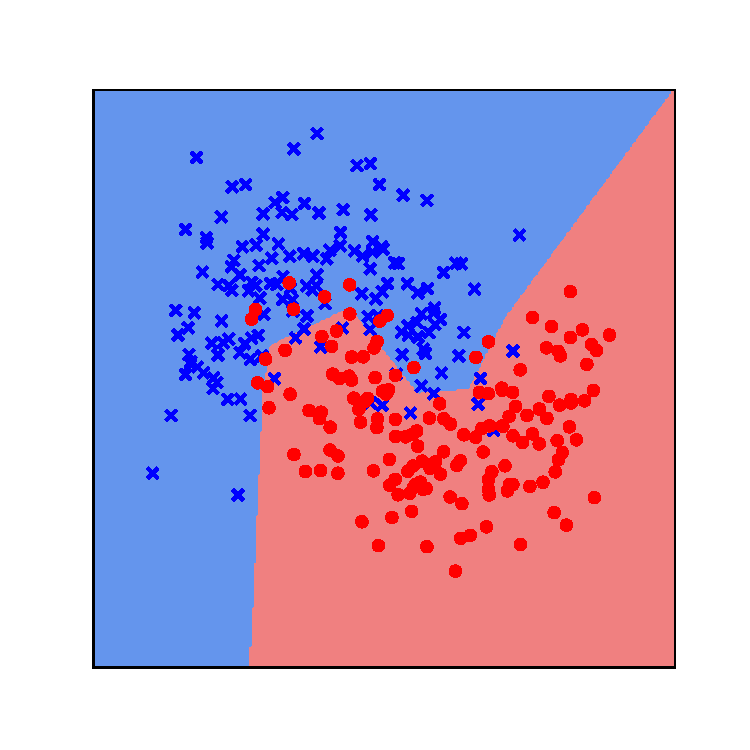
\includegraphics[width=0.98\textwidth]{figures/main/ch2-background/normal.pdf}
    \caption{Good fit}
    \label{figure:ch2-fitting_points_c}
  \end{subfigure}
  \caption{
    Decision boundary of 3 classifiers with different complexity for the same set of sample.
  }
  \label{figure:ch2-fitting_points}
\end{figure}


A fundamental question remains: \emph{how to choose the correct hypothesis class for which $\text{ERM}_\mathcal{H}$ will not lead to overfitting?} 
We answer this question by decomposing the true risk into two different components as follows: 
\begin{equation}
  R_\mathcal{D} (h_\mathcal{S}) = 
  \underbrace{\left[ \min_{h \in \mathcal{H}} R_\mathcal{D}(h) \right]}_{\text{\scriptsize Approximation Error}} + \quad 
  \underbrace{\left[ R_\mathcal{D}(h_\mathcal{S}) - \min_{h \in \mathcal{H}} R_\mathcal{D}(h) \right]}_{\text{\scriptsize Estimation Error}} 
  \label{equation:ch2-bias_complexity_tradeoff}
\end{equation}
\begin{itemize}
  \item \textbf{Approximation Error}: The approximation error corresponds to the minimum risk achievable by a classifier in the given hypothesis class.
  Intuitively, this error measure the quality of the hypothesis class and therefore the quality of the prior knowledge.
  Enlarging the hypothesis class, \ie, allowing more complex functions, can decrease the approximation error.
  \item \textbf{Estimation Error}: The estimation error is the difference between the approximation error and the error made by the ERM predictor.
  Recall that the empirical risk is only an estimate of the true risk.
  This error is dependent on the sample size and/or the complexity of the hypothesis class. 
\end{itemize}
Recall that the main goal is to minimize the true risk $R_\mathcal{D} (h_\mathcal{S})$, however, Equation~\ref{equation:ch2-bias_complexity_tradeoff} shows a tradeoff called the \emph{bias-complexity tradeoff}. 
The tradeoff is as follows: if we choose a large and complex hypothesis space, we reduce the approximation error but at the same time can increase the estimation error because a complex hypothesis space might lead to overfitting.
Conversely, choosing a small hypothesis space might reduce the estimation error but increase the approximation error leading to an \emph{underfitting} phenomenon.
We can demonstrate the \emph{overfitting} and \emph{underfitting} phenomenons with Figure~\ref{figure:ch2-fitting_points} which shows the decision boundary of 3 classifiers for the same set of samples.
Figure~\ref{figure:ch2-fitting_points_a} shows a classifier which \emph{underfit} the data, meaning the decision boundary is not complex enough to separate the data correctly. 
The Figure~\ref{figure:ch2-fitting_points_b} shows a classifier that almost perfectly follows the training data but is likely to have a higher error rate on the unseen data.
Finally, the Figure~\ref{figure:ch2-fitting_points_c} shows a classifier that seems to have a good compromise between the two.

As seen above, defining a small hypothesis class might lead to underfitting and a large hypothesis class might lead to overfitting.
A good way to offset a large hypothesis class would be to specific preference over hypothesis within the hypothesis class.
The \emph{Structural Minimization Paradigm} (SRM) assumes that the hypothesis class can be written as the union of multitude smaller hypothesis class as follows: $\mathcal{H} = \bigcup_{n \in \Nbb} \mathcal{H}_n$ with a weight function $w: \Nbb \rightarrow [0, 1]$ which assigns a weight to each hypothesis class, $\mathcal{H}_n$, such that a higher weights reflects a lower preference for the hypothesis class.
Intuitively, the weight function is a measure of the ``complexity'' of the hypotesis.
The SRM learning paradigm can then be defined as follows:
\begin{equation}
  \text{SRM}_\mathcal{H} \in \argmin_{h \in \mathcal{H}, n \in \Nbb} \left[ R_\mathcal{S}(h) + w(n) \right]
\end{equation}
The SRM learning paradigm minimizes the empirical risk $R_\mathcal{S}(h)$ and the weight function $w$; therefore, ovoiding overfitting and improving generalization by reducing the complexity of the hypotesis while maintening a low empirical risk. 
% In the next section, we will present neural networks which are the type of function we will use as predictors and we will see how to implement the ERM and SRM paradigm.









% \‰\‰\‰
%
% The ERM paradigm with inductive bias is based on an important assumption.
% We assume that uniformly over all $h \in \mathcal{H}$, the empirical risk is close to the true risk, meaning, an $h$ that minimize the empirical risk with respect to a data set $\mathcal{S}$ will also minimize the \emph{true} risk.
% More formally, 
% \begin{equation}
%   \forall h \in \mathcal{H}, \quad \left| R_\mathcal{S}(h) - R_\mathcal{D}(h) \right| \leq \epsilon \enspace.
%   \label{equation:ch2-eps_respresentative_sample} 
% \end{equation}
% If this assumption is met, then the ERM paradigm will always return a good classifier. 
% \begin{lemma}[Lemma 4.2 \citet{shalev2014understanding}] 
%   If Equation~\ref{equation:ch2-eps_respresentative_sample} hold, then any output of $\mathrm{ERM}_\mathcal{H}(\mathcal{S})$, namely, any $h_\mathcal{S} \in \argmin_{h \in \mathcal{H}} R_\mathcal{S}(h)$, satisfies
%   \begin{equation}
%     R_\mathcal{D}(h_\mathcal{S}) \leq \min_{h \in \mathcal{H}} R_\mathcal{S}(h) + 2\epsilon
%   \end{equation}
% \end{lemma}
%
% \‰\‰\‰


% Let us consider an input space $\mathcal{X} = [0, 1]^d$ of dimension $d$, an output space $\mathcal{Y} = [k]$ where $k$ is the number of class and a data distribution $\mathcal{D}$ over $\mathcal{X} \times \mathcal{Y}$.
% We seek to find a function $h: \mathcal{X} \rightarrow \mathcal{Y}$ that maps the input $\xvec \in \mathcal{X}$ to the output $y \in \mathcal{Y}$ with $h \in \mathcal{H}$ where $h$ is called the \emph{hypothesis} and $\mathcal{H}$ the \emph{hypothesis space}.
% in order to measure how well the function fits, we de\emph{loss function} $l: \mathcal{y} \times \mathcal{y} \rightarrow \rbb^{+}$ is defined.
% The \emph{risk} $R$ associated with the hypothesis $h(\xvec)$ is defined as follows:
% \begin{equation}
%   R(h) \triangleq \Ebb_{(\xvec, y) \sim \mathcal{D}}\  L \left( h(\xvec), y \right)
% \end{equation}
% The goal of a \emph{learning algorithm} is to find a hypothesis $h^* \in \mathcal{H}$ which minimize the risk $R(h)$:
% \begin{equation}
%   h^* \triangleq \argmin_{h \in \mathcal{H}} R(h) .
% \end{equation}

% In practice, the joint probability distribution $\mathcal{D}$ is unknown.
% Instead, we have $n$ independent observations of the distribution called the \emph{training set}
% \begin{equation}
%   \mathcal{T} \triangleq \left\{ \left(\xvec^{(1)}, y^{(1)} \right), \dots, \left( \xvec^{(n)}, y^{(n)} \right) \right\} ,
% \end{equation}
% where $\xvec \in \mathcal{X}$ and $y \in \mathcal{Y}$.

% The risk minimization problem is therefore replace by the \emph{empirical risk minimization} as follows:
% \begin{equation}
%   E(h, n) \triangleq \frac{1}{n} \sum_{i = 1}^{n} L\left(h\left(\xvec^{(i)}\right), y^{(i)}\right) ,
% \end{equation}
% the learning algorithm then becomes:
% \begin{equation}
%   \hat{h}^* \triangleq \argmin_{h \in \mathcal{H}} E(h, n)  .
% \end{equation}


% \paragraph{Structural Risk Minimization} (SRM).
% The ERM principle assumes that the function $\hat{h}^*$ minimizing $E(h, n)$ leads to the risk $R(\hat{h}^*)$ being close to the minimum.
% This assumption mean that as the \emph{size} of the training set increase the minimization becomes more accurate. More formally, the ERM principle assumes that $R(\hat{h}^*)$ converge to its minimum value on the set $h \in \mathcal{H}$ when $n \rightarrow \infty$.  
% \citet{Vapnik1991TheNA} have shown that this equivalent to say that the empirical risk $E(h, n)$ \emph{converge uniformly} to the actual risk $R(h)$ over $h \in \mathcal{H}$ where the \emph{uniform convergence} is defined as follows:
% \begin{equation}
%   \Pbb \left[ \sup_{h \in \mathcal{H}} \left| R(h) - E(h, n) \right| < \epsilon \right] \rightarrow 0 \quad \text{ when } \quad n \rightarrow \infty, \quad \forall \epsilon > 0 
% \end{equation}


% \citet{Vapnik1991TheNA} have shown that this assumption is equivalent to the following: does the empirical risk $E(h, n)$ \emph{converge uniformly} to the actual risk $R(h)$ over $h \in \mathcal{H}$ where the \emph{uniform convergence} is defined as follows:
% \begin{equation}
%   \Pbb \left[ \sup_{h \in \mathcal{H}} \left| R(h) - E(h, n) \right| < \epsilon \right] \rightarrow 0 \quad \text{ when } \quad n \rightarrow \infty, \quad \forall \epsilon > 0 
% \end{equation}


% However, does increasing the \emph{size} of the training set allow a better minimisation of the actual risk. More formally, does $R(\hat{h}^*)$ converge to its minimum value on the set $h \in \mathcal{H}$ when $n \rightarrow \infty$. 

% \citet{vapnik1992principles} 

% The 0-1 loss function is a natural loss function to use because it assigns 0 for a correct classification and 1 for an incorrect classification. 


% of the ERM principle \ie, does $R(\hat{h}^*)$ converge to its minimum value on the set $h \in \mathcal{H}$ when $n \rightarrow \infty$ is equivalent to the question: 

% is equivalent to the question: does the empirical risk E(h, n) \emph{converge uniformly} to the actual risk $R(h)$ over $h \in \mat

% \begin{equation}
%   h^* = \argmin_{h \in \mathcal{H}} \frac{1}{n} \sum_{i = 0}^{n} L(h(\xvec_i), y) + \lambda C(\theta) 
% \end{equation}

% Because the relation between $\xvec \in \mathcal{X}$ and $y \in \mathcal{Y}$ is unknown, we aim to find the best approximation of the function $h$ with a parameterized function $h_\theta \in \mathcal{H}$ where $\mathcal{H}$ is called the \emph{hypothesis space}.

% The goal of a \textbf{learning algorithm} is to learn a function $f: \mathcal{X} \rightarrow \mathcal{Y}$ which outputs $y \in \mathcal{Y}$ given an input $\xvec \in \mathcal{X}$ with $f \in \mathcal{H}$ where $\mathcal{H}$ is called the \emph{hypothesis space}.

% The supervised learning settings assume that a function $f: \mathcal{X} \rightarrow \mathcal{Y}$ exists. 

% The supervised learning settings assume that a function $f$ that maps $\xvec \sim \mathcal{X}$ to $y \sim \mathcal{y}$ exists. 

% The goal of a \textbf{learning algorithm} is to approximate $f$ by a parameterized function $f_\theta$.
% The standard method to learn the set of parameters $\theta$ is the \textbf{empirical risk minimization (ERM)}:
% \begin{equation*}
%   \hat{\theta}_{ERM} \triangleq \argmin_{\theta} \frac{1}{n} \sum_{i=1}^{n} L (f_{\theta} (\xvec_i), y_i )
% \end{equation*}

% \begin{equation}
%   \min_{\theta} \Ebb_{(\xvec, y) \sim \mathcal{D}} \left[ L(f_\theta(x), y) \right]. 
% \end{equation}


%%%%%%%%%%%%%%%%%%%%%%%%%%%%%%%%%%%%%%%%%%%%%%%%%%%%%%%%%%%%%%%%%%%%%%%%%%%%%%%
\section{Preliminaries on Neural Networks}
\label{subsection:ch2-neural_networks}
%%%%%%%%%%%%%%%%%%%%%%%%%%%%%%%%%%%%%%%%%%%%%%%%%%%%%%%%%%%%%%%%%%%%%%%%%%%%%%%


In the previous section, we said that we restrict the learner towards a specific set of predictors.
In this thesis, we will focus on neural networks. 
Neural networks, which find their roots in the work of \citet{mcculloch1943logical,rosenblatt1958perceptron}, can be analytically described as a composition of linear functions interlaced with non-linear functions (also called activation functions).
A neural network can be defined as follows:

% \begin{definition}[Neural Network]
%   Given a depth $\depth \in \Nbb$, 
%   let $w = \{ w^{(i)} \}_{i \in [\depth]}$ and $b = \{ b^{(i)} \}_{i \in [\depth]}$ be sequences of ``dimension'',  
%   $\weights = \left\{ \left( \Wmat^{(i)}, \bvec^{(i)} \right) \right\}_{i \in [\depth]}$ a set of weights matrices and bias vectors 
%   such that $\Wmat^{(i)} \in \Rbb^{w^{(i)}}$ and $\bvec^{(i)} \in \Rbb^{b^{(i)}}$ and 
%   sequence of activation functions $\act = \{\act_i \}_{i \in [\depth]}$.
% %   Let $\dim^{w} = \{ \dim_1^w, \dots, \dim_\depth^w \}$ and $\dim^{b} = \{ \dim_1^b, \dots, \dim_\depth^b \}$ 
% % be sequences of ``dimension'', let $\dim_{\text{in}} = \dim_\depth^w$ and $\dim_{\text{out}} = \dim_\depth^w$.
%   Let $\mathcal{X} \subset \Rbb^{\dim_{\text{in}}}$ and 
%   $\mathcal{Y} \subset \Rbb^{\dim_\text{out}^w}$ be the input space and output space respectively. 
%   % Given a depth $\depth$, a set of weights matrices and bias vectors $\weights = \left\{ \left( \Wmat^{(i)}, \bvec^{(i)} \right) \right\}_{i \in [\depth]}$ and a sequence of activation functions $\act = \{\act_i \}_{i \in [\depth]}$, a neural network is a function $N^\act_\weights : \mathcal{X} \rightarrow \mathcal{Y}$ such that
%   A neural network is a function $N^\act_\weights : \mathcal{X} \rightarrow \mathcal{Y}$ such that
%   \begin{equation}
%     \nn^\act_{\weights}(\xvec) \triangleq \phi^{\act_\depth}_{\Wmat^{(\depth)}, \bvec^{(\depth)}} \circ \cdots \circ \phi^{\act_1}_{\Wmat^{(1)}, \bvec^{(1)}}(\xvec)
%   \end{equation}
%   % where $d$ corresponds to the depth of the network (\ie, the number of layers), $\weights$ is the set of weights matrices and bias vectors $\weights = \left\{ \left( \Wmat^{(1)}, \bvec^{(1)} \right) \dots \left( \Wmat^{(d)}, \bvec^{(d)} \right) \right\}$.
%   % $\Bmat$ is the set of bias vectors $\Bmat = \left\{ \right\}$. 
%   where $\phi^{\act_i}_{\Wmat^{(i)},\bvec^{(i)}}: \Rbb^{w^{(i)}} \rightarrow \Rbb^{w^{(i+1)}}$ (also called layer) is a function parameterized by the weight matrix $\Wmat^{(i)}$, the bias vector $\bvec^{(i)}$ and the activation function $\act_i$ and can be expressed as follows: 
%   \begin{equation}
%     \phi^{\act_i}_{\Wmat^{(i)},\bvec^{(i)}} (\xvec) \triangleq \act_i \left(\Wmat^{(i)}\xvec + \bvec^{(i)}\right)
%   \end{equation}
% \end{definition}

\begin{definition}[Neural Network]
  Given a depth $\depth \in \Nbb$, 
  let $\dimw = \{ \dimw^{(i)} \}_{i \in [\depth]}$ and $\dimb = \{ \dimb^{(i)} \}_{i \in [\depth]}$ be sequences of ``dimension'', $\weights = \left\{ \left( \Wmat^{(i)}, \bvec^{(i)} \right) \right\}_{i \in [\depth]}$ a set of weights matrices and bias vectors 
  such that $\Wmat^{(i)} \in \Rbb^{\dimw^{(i)}}$ and $\bvec^{(i)} \in \Rbb^{\dimb^{(i)}}$ and sequence of activation functions $\act = \{\act_i \}_{i \in [\depth]}$.
  Let $\mathcal{X} \subset \Rbb^{\dimw^{(1)}}$ and $\mathcal{Y} \subset \Rbb^{\dimw^{(\depth)}}$ be the input space and output space respectively. 
  $\dimw^{(1)}$ refer to the input dimension and $\dimw^{(\depth)}$ refer to the output dimension.
  
  \noindent
  A neural network is a function $\nn^\act_\weights : \mathcal{X} \rightarrow \mathcal{Y}$ such that
  \begin{equation}
    \nn^\act_{\weights}(\xvec) \triangleq \phi^{\act_\depth}_{\Wmat^{(\depth)}, \bvec^{(\depth)}} \circ \cdots \circ \phi^{\act_1}_{\Wmat^{(1)}, \bvec^{(1)}}(\xvec)
  \end{equation}
  where $\phi^{\act_i}_{\Wmat^{(i)},\bvec^{(i)}}: \Rbb^{w^{(i)}} \rightarrow \Rbb^{w^{(i+1)}}$ (also called layer) is a function parameterized by the weight matrix $\Wmat^{(i)}$, the bias vector $\bvec^{(i)}$ and the activation function $\act_i$ and can be expressed as follows: 
  \begin{equation}
    \phi^{\act_i}_{\Wmat^{(i)},\bvec^{(i)}} (\xvec) \triangleq \act_i \left(\Wmat^{(i)}\xvec + \bvec^{(i)}\right)
  \end{equation}
\end{definition}



\noindent
Based on this definition, for a given training set $\mathcal{S} = \mathcal{X} \times \mathcal{Y}$, a set of activation functions $\act$, a set of weights and biases $\weights$ and a loss function $L: \mathcal{Y} \times \mathcal{Y} \rightarrow \Rbb_+$, the ERM learning paradigm for neural networks is given by
\begin{equation}
  \argmin_{\weights} \frac{1}{|\mathcal{S}|} \sum_{(\xvec, y) \in \mathcal{S}} L(N^\act_\weights(\xvec), y) 
  \label{equation:ch2-erm_neural_network}
\end{equation}
For classification problem, the zero-one loss is known to be non-convex and non-smooth, and it has been shown that solving for the optimal solution is an NP-hard combinatorial optimization problem~\cite{feldman2012agnostic,bendavid2003difficulty}.
Instead, a common approach is to used the softmax activation function as the last non-linear activation $\act_d$ with the cross-entropy loss function and estimate the parameters with \emph{maximum likelihood}~\cite{hastie2009elements}.
The softmax activation function, $\act_d: \Rbb^k \rightarrow [0, 1]^k$, is defined as follows:
\begin{equation}
  \leftmat \act_d(\xvec) \rightmat_i = \frac{e^{\xvec_i}}{\sum_{j=0}^{k-1} e^{\xvec_j}}, \quad \forall i \in [k-1]_0
\end{equation}
The generic approach for minimizing the empirical risk in Equation~\ref{equation:ch2-erm_neural_network} is by \emph{gradient descent} with the \emph{backpropgation} algorithm ~\cite{rumelhart1986learning} which consists of computing the gradient with the help of the chain-rule.


As seen in the previous section, the SRM paradigm minimizes two terms, the empirical risk and a weight function measuring the ``complexity'' of the hypothesis.
% It has been shown that the number of free parameters can be used as a measure of complexity and a number of work have proposed techniques to reduce the number parameters~\cite{lecun1990optimal,thodberg1991improving,weigend1991generalization}.
% However, a different way of constraining the complexity is to limit the growth of weights~\cite{hinton1987learning}.
% This \emph{regularization} \cite{tikhonov1977solutions,krogh1992simple}, also called \emph{weight decay}, prevents weights from growing too large unless it is necessary.
It has been shown that the $\ell_2$ norm of the weights of a network can be used as a measure of complexity; therefore, limiting the growth of the weights constraints the complexity of the network ~\cite{hinton1987learning}.
% However, a different way of constraining the complexity is to limit the growth of weights~\cite{hinton1987learning}.
This \emph{regularization} \cite{tikhonov1977solutions,krogh1992simple}, also called \emph{weight decay}, prevents weights from growing too large unless it is necessary.
The SRM learning algorithm with the weight decay regularization can be expressed as follows:
\begin{equation}
  \argmin_{\weights} \frac{1}{|\mathcal{S}|} \sum_{(\xvec, y) \in \mathcal{S}} L(N^\act_\weights(\xvec), y) + \lambda \sum_{(\Wmat, \bvec) \in \weights} \left( \norm{\Wmat}_\mathrm{F} + \norm{\bvec}_\mathrm{2} \right)
\end{equation}
where $\lambda > 0$ is the regularization parameter.



\begin{figure}[htb]
  \centering
  \begin{subfigure}[b]{0.32\textwidth}
    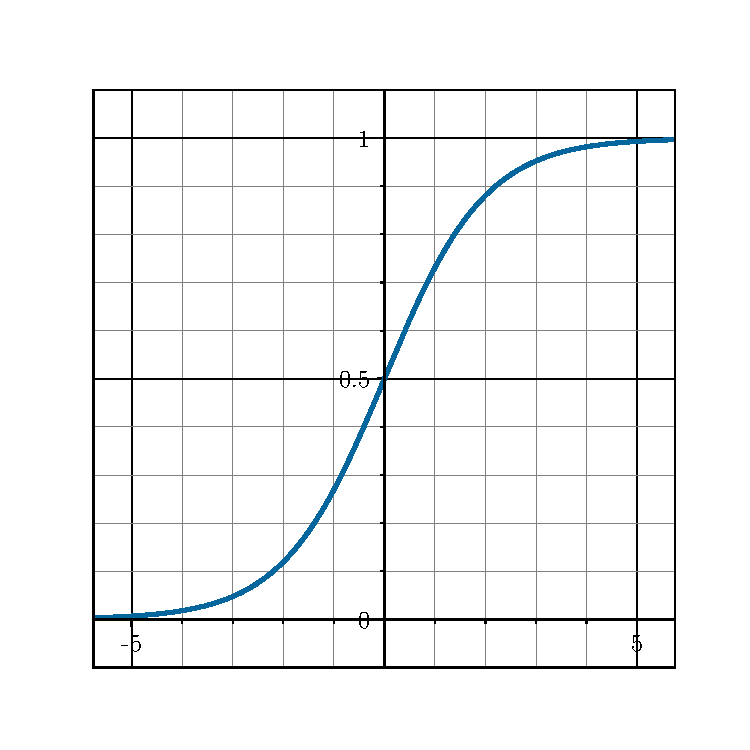
\includegraphics[width=0.98\textwidth]{figures/main/ch2-background/sigmoid.pdf}
    \caption{Sigmoid Activation}
  \end{subfigure}
  \hfill
  \begin{subfigure}[b]{0.32\textwidth}
    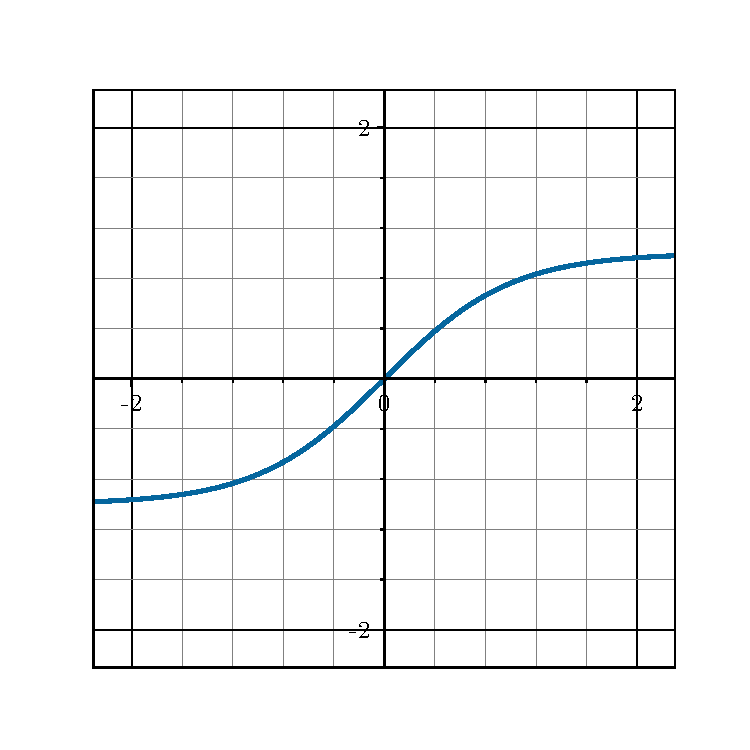
\includegraphics[width=0.98\textwidth]{figures/main/ch2-background/tanh.pdf}
    \caption{Tanh Activation}
  \end{subfigure}
  \hfill
  \begin{subfigure}[b]{0.32\textwidth}
    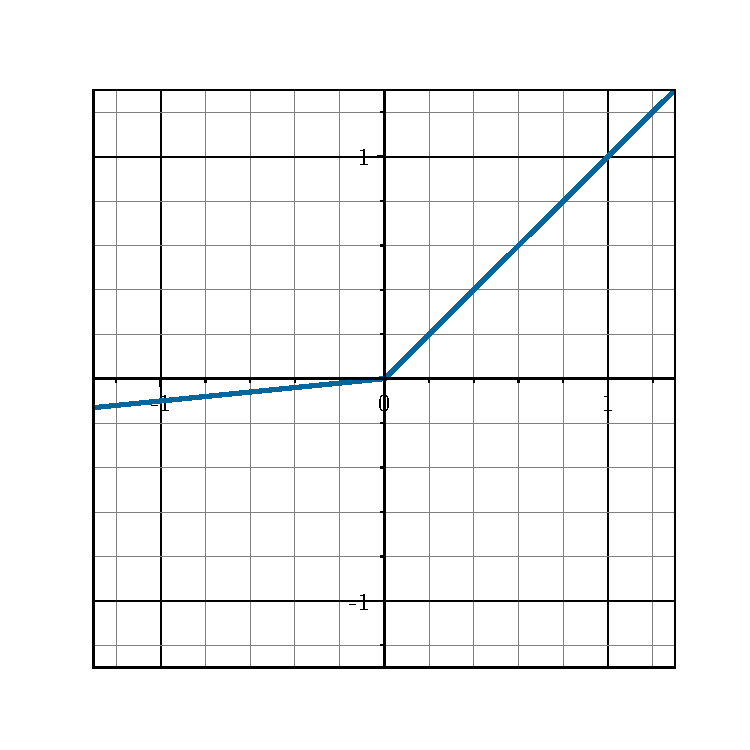
\includegraphics[width=0.98\textwidth]{figures/main/ch2-background/relu.pdf}
    \caption{Leaky ReLU Activation}
  \end{subfigure}
  \caption{Graphical representation of 3 common activation functions}
  \label{figure:ch2-activation_functions}
\end{figure}


Choosing the right activation function has been an active area of research. 
Hereafter, we present 3 common activation functions used by practitioners.
\begin{itemize}
  \item \textbf{Sigmoid activation} \cite{han1995influence}
    \begin{equation*}
      \act(x) = \frac{1}{1+e^{-x}} 
    \end{equation*}
    The sigmoid activation function is one of the first continuous non-linear function to be used in the context of neural network. It takes a real value as input and outputs another value between 0 and 1.
  \item \textbf{Hyperbolic Tangent activation} \cite{karlik2011performance}
    \begin{equation*}
      \act(x) = \frac{e^x - e^{-x}}{e^x + e^{-x}}
    \end{equation*}
    The hyperbolic tangent activation function is similar to the sigmoid activation function but instead of returning between 0 and 1, the function returns between -1 and 1.     
  \item \textbf{Leaky Rectified Linear activation (Leaky-ReLU)} \cite{maas2013rectifier}
    \begin{equation*}
      \act(x) = \max(\alpha, x)
    \end{equation*}
    More recently, the ReLU~\cite{nair2010rectified} ($\alpha = 0$) and leaky-ReLU~\cite{maas2013rectifier} ($\alpha > 0$) activation function was proposed.
    The parameter $\alpha$ characterize the slope on $\Rbb_-$.
    These function have the advantages to avoids the vanishing gradient problem and are less less computationally expensive than tanh and sigmoid because it involves simpler mathematical operations.
\end{itemize}

\noindent
The Figure~\ref{figure:ch2-activation_functions} present the graphical representation of the 3 activation functions presented above.
In this thesis, we will exclusively use the Leaky-ReLU function with different $\alpha$ when we train deep neural networks.
Therefore, we simplify the notation $\nn^\act_\weights$ with $\nn_\weights$.


The architecture of a neural network is governed by mainly two factors: the dimensions of the hidden layers and the depth of the network.
Different types of scaling have been studied.
Neural networks with large width have been studied both theoretically and experimentally.
\citet{cybenko1989approximation,hornik1989multilayer} have shown that neural networks with a single hidden layer and sigmoid activation can approximate any function if the hidden layer is allowed to be arbitrary large. 
However, wide and shallow networks tend to be difficult to train due to having difficulties in capturing higher-level features. 
Indeed, it has been empirically observed that deep neural networks tend to achieve greater performance that large and shallow neural networks.
More recently, the \emph{universal approximation result} have been extended to bounded width neural network with arbitrary depth~\cite{lu2017expressive,hanin2017universal}.
More formally, we have the following result for neural networks with $\relu$ activations:
\begin{theorem}[Universal Approximation Theorem for Neural Network \citet{hanin2017universal}]
  For any continuous function $f:[0,1]^{n} \rightarrow \mathbb{R}_+$ of bounded supremum norm, for any $\epsilon>0$, there exists a neural network $\nn_\weights$ parametried by $\weights$ with an input layer of width $n$, an output layer of width $1$, hidden layers of width $n+3$ and ReLU activations such that 
  \begin{equation}
    \forall x \in [0,1]^n, \quad \left| f(\xvec) - \nn_\weights(\xvec) \right| < \epsilon \enspace.
  \end{equation}
\end{theorem}



% From $\mathcal{N}$, we can easily build a deep ReLU network $\mathcal{N'}$ of width exactly $n+3$, such that $\forall x \in [0,1]^{n+3}$, $\left|f(\xvec_{1} \ldots \xvec_{n}) - \left(\mathcal{N}'\left(\xvec\right)\right)_{1}\right| < \epsilon$. Thanks to Lemma~\ref{lemma:dcnn_approx_neural_network}, this last network can be approximated arbitrarily well by a DCNN of width $n+3$.
%
% \begin{theorem}
%   Let $\mathcal{X} \subset \Rbb^{w_{(1)}}$.
%   For any continuous function $f: \mathcal{X} \rightarrow \Rbb^{w^{(\depth)}}$, then there exists a  
%
%   Let $\mathcal{X} \subset \Rbb^{w_{(1)}}$ and let $f: \Rbb^{w^{(1)}} \rightarrow \Rbb^{w^{(\depth)}}$ be a continuous function.
%   Then, there exists a neural networks parameterized by $\weights$ with an input dimension $w^{(1)}$, an arbitrary depth $\depth$, and $\relu$ activation such that:
%   \begin{equation}
%     \norm{f(\xvec) - \nn(\xvec)} \leq \epsilon
%   \end{equation}
%   \label{theorem:ch2-universal_approximation_theorem}
% \end{theorem}
%


% \citet{cybenko1989approximation} have shown that shallow neural networks with sigmoid activation can \emph{theoretically} approximate any decision boundary.
%
% The arbitrary depth case was also studied by number of authors, such as Zhou Lu et al in 2017,[11] 
% \cite{lu2017expressive}
%
% Boris Hanin and Mark Sellke in 2018,[12] 
% \cite{hanin2017universal}





%%%%%%%%%%%%%%%%%%%%%%%%%%%%%%%%%%%%%%%%%%%%%%%%%%%%%%%%%%%%%%%%%%%%%%%%%%%%%%%
\section{Adversarial Attacks \& Robustness of Neural Networks}
\label{section:ch2-preliminaries_on_adversarial_attacks}
%%%%%%%%%%%%%%%%%%%%%%%%%%%%%%%%%%%%%%%%%%%%%%%%%%%%%%%%%%%%%%%%%%%%%%%%%%%%%%%

As seen in the introduction (Chapter \ref{chapter:ch1-introduction}), deep neural networks achieve state-of-the-art performances in a variety of domains such as natural language processing~\cite{radford2018Language}, image recognition~\cite{he2016deep} and speech recognition~\cite{hinton2012deep}.
However, it has been shown that such neural networks are vulnerable to \emph{adversarial examples}, \ie, imperceptible variations of the natural examples, crafted to deliberately mislead the models~\cite{globerson2006nightmare,biggio2013evasion,szegedy2013intriguing}.
Because it is difficult to characterize the space of visually imperceptible variations of a natural image, existing adversarial attacks use $\ell_p$ norms as surrogates measure.
We can formally define an adversarial example as follows:
\begin{definition}[Adversarial Pertubation]
  Given a dataset $\mathcal{S} = \mathcal{X} \times \mathcal{Y}$, a pair $(\xvec, y) \sim \mathcal{S}$ and a trained neural network $\nn_\weights$ on $\mathcal{S}$ such that $\argmax_{i \in [k-1]_0} \{ \nn_\weights(\xvec)_i \} = y$, let $\adv \in \mathcal{X}$ be an adversarial perturbation such that:
  \begin{align}
    &\argmax_{i \in [k-1]_0} \{ \nn_\weights (\xvec + \adv)_i \} \neq y \\
    \st\ &\norm{\adv}_p \leq \epsilon \notag
  \end{align}
  where $\epsilon$ is a small value defined by the attacker. 
\end{definition}

%%%%%%%%%%%%%%%%%%%%%%%%%%%%%%%%%%%%%%%%%%%%%%%%%%%%%%%%%%%%%%%%%%%%%%%%%%%%%%%
\subsection{Implementing Adversarial Attacks}
\label{subsection:ch2-adversarial_attacks}
%%%%%%%%%%%%%%%%%%%%%%%%%%%%%%%%%%%%%%%%%%%%%%%%%%%%%%%%%%%%%%%%%%%%%%%%%%%%%%%

\noindent
Since the discovery of adversarial perturbations, a variety of procedures, \aka \emph{adversarial attack}, have been developed to generate adversarial examples, for example FGSM \cite{goodfellow2014explaining}, PGD \cite{madry2018towards} and C\&W \cite{carlini2017towards}, to mention the most popular ones.
To find the best perturbation $\adv$, existing attacks can adopt one of the two following strategies:
\begin{itemize}
  \item \textbf{Loss maximization}: maximizing the loss $L(\nn_\weights(\xvec + \adv), y)$ under some constraint on $\norm{\adv}_p$ with $p \in \{0, \dots, \infty\}$.;
  \item \textbf{Perturbation minimization}: minimizing $\norm{\adv}_p$ under some constraint on the loss $L(\nn_\weights(\xvec + \adv), y)$.
\end{itemize}

\paragraph{Loss maximization.}
In this scenario, the procedure maximizes the loss objective function, under the constraint that the $\lp$ norm of the perturbation remains bounded by some value $\epsilon$, as follows:  
\begin{equation}
  \argmax_{\adv:\norm{\adv}_p \leq \epsilon} L(\nn_\weights(\xvec + \adv), y) \enspace.
  \label{equation:ch2-lossmax}
\end{equation}
The typical value of $\epsilon$ depends on the norm $\norm{\ \cdot\ }_p$ considered in the problem setting.
% In order to compare $\linf$ and $\ltwo$ attacks of similar strength, we choose values of $\epsilon_\infty$ and $\epsilon_2$ (for $\linf$ and $\ltwo$ norms respectively) which result in $\linf$ and $\ltwo$ balls of equivalent volumes.
% For the particular case of CIFAR-10, this would lead us to choose $\epsilon_\infty = 0.03$ and $\epsilon_2 = 0.8$ which correspond to the maximum values chosen empirically to avoid the generation of visually detectable perturbations. 
The current state-of-the-art method to solve Equation~\ref{equation:ch2-lossmax} is based on a projected gradient descent (PGD)~\cite{madry2018towards} of radius~$\epsilon$.
Given a budget $\epsilon$, it recursively computes
\begin{equation}
  \xvec^{(t+1)} = \prod_{\mathcal{B}_p(\xvec,\epsilon)}\left(\xvec^{(t)}
    + \alpha \argmax_{\adv: \norm{\adv}_p \leq 1} \nabla_\xvec L\left( \nn_\weights \left(\xvec^{(t)} + \adv \right), y \right)
\right)
  \label{equation:ch2-projectionPGD}
\end{equation}
where $\mathcal{B}_p(\xvec,\epsilon) = \{ \xvec + \adv:\norm{\adv}_p \leq \epsilon\}$, $\alpha$ is a gradient step size, and $\prod_S$ is the projection operator on $S$.
The PGD attack is currently used in the literature with $p=2$ and $p=\infty$.
The attack with the norm $p=\infty$ is state-of-the-art for the loss maximization problem. 

\paragraph{Perturbation minimization.}
This type of procedure search for the perturbation that has the minimal $\lp$ norm, under the constraint that $L(\nn_\weights(\xvec + \adv), y)$ is bigger than a given bound $c$:
\begin{align}
  &\argmin_{\adv} \norm{\adv}_p \label{equation:ch2-normmin} \\
  \st\ &L(\nn_\weights(\xvec + \adv), y) \geq c \notag
\end{align}
The value of $c$ is typically chosen depending on the loss function $L$. For example, if $L$ is the $0-1$ loss, any $c > 0$ is acceptable.
Equation~\ref{equation:ch2-normmin} has been tackled by~\citet{carlini2017towards}, leading to the following method, denoted C\&W attack in the rest of the chapter. It aims at solving the following Lagrangian relaxation of Equation~\ref{equation:ch2-normmin}:
\begin{equation}
  \argmin_{\adv} \norm{\adv}_p + \lambda g(\xvec+\adv)
\end{equation}
where $g(\xvec + \adv)<0$ if and only if $L(\nn_\weights(\xvec + \adv),y) \geq c$. 
The authors use a change of variable $\adv = \tanh(\wvec) - \xvec$ to ensure that $\xvec + \adv \in \mathcal{X}$, a binary search to optimize the constant $c$, and Adam or SGD to compute an approximated solution.
The C\&W attack is currently used in the literature with $p \in \{1, 2, \infty \}$ and is state-of-the-art with $p=2$ for the perturbation minimization problem
% This attack with the norm $p=2$ is state-of-the-art for the perturbation minimization problem. 
% The C\&W attack is well defined both for $p=2$, and $p=\infty$, but there is a clear empirical gap of efficiency in favor of the $\ltwo$ attack.


% For example, \citet{goodfellow2014explaining} use the $\linf$ norm to measure the distance between the original image and the adversarial image whereas \citet{carlini2017towards} use the $\ltwo$ norm.
% When the input dimension is low, the choice of the norm is of little importance because the $\linf$ and $\ltwo$ balls overlap by a large margin, and the adversarial examples lie in the same space.
% For typical image datasets with large dimensionality, the two balls are mostly disjoint.
% As a consequence, the $\linf$ and the $\ltwo$ adversarial examples lie in different areas of the space, and it explains why $\linf$ defense mechanisms perform poorly against $\ltwo$ attacks and vice versa. 



%%%%%%%%%%%%%%%%%%%%%%%%%%%%%%%%%%%%%%%%%%%%%%%%%%%%%%%%%%%%%%%%%%%%%%%%%%%%%%%
\subsection{Defending against Adversarial Attacks}
\label{subsection:ch2-defending_against_adversarial_attacks}
%%%%%%%%%%%%%%%%%%%%%%%%%%%%%%%%%%%%%%%%%%%%%%%%%%%%%%%%%%%%%%%%%%%%%%%%%%%%%%%

Given the important security risks that adversarial attacks pose, it is important to design defenses to protect neural networks against these kinds of attacks.
Adversarial Training was introduced by~\citet{goodfellow2014explaining} and later improved by~\citet{madry2018towards} as a first defense mechanism to train robust neural networks.
It consists in augmenting training batches with adversarial examples generated during the training procedure.
The structural risk minimization paradigm is thus replaced by the following $\min$ $\max$ problem, where the classifier tries to minimize the expected loss under maximum perturbation of its input:
\begin{equation}
  \argmin_\weights \argmax_{\adv: \norm{\adv} \leq \epsilon} \frac{1}{|\mathcal{S}|} \sum_{(\xvec, y) \in \mathcal{S}} L\left( \nn_\weights \left(\xvec + \adv \right), y \right) + \lambda \sum_{(\Wmat, \bvec) \in \weights} \left( \norm{\Wmat}_\mathrm{F} + \norm{\bvec}_\mathrm{2} \right)
\end{equation}
% In the case where $p = \infty$, this technique offers good robustness against $\linf$ attacks \cite{athalye2018obfuscated}.
Although adversarial training lacks formal guarantees, it is one of the few techniques that prove to be empirically very effective.


% Despite some recent work providing great insights \cite{sinha2017certifying,zhang2019theoretically}, there is no worst case lower bound yet on the accuracy under attack of this method.




% \%\%\%
%
% \cite{goodfellow2014explaining} have proposed \textbf{Adversarial Training} which follows \textbf{ERM} training over adversarially-perturbed samples
%
%
% \%\%\%

% Another important technique to defend against adversarial examples is to use \emph{noise injection} techniques.  
% In contrast with adversarial Training, noise injection mechanisms are usually deployed after training.


% In a nutshell, it works as follows.
% At inference time, given a unlabeled sample $x$, the network outputs
% \begin{equation}
%   \tilde{f}_\theta(\xvec) \triangleq f_\theta(\xvec + \eta) \ \ \ (\text{instead of  } f_\theta(\xvec)) 
% \end{equation}
% where $\eta$ is a random variable on $\mathbb{R}^d$.
% Even though, Noise Injection is often less efficient than Adversarial Training in practice (see \eg, Table~\ref{table:764774}), it benefits from strong theoretical background.
% In particular, recent works \cite{lecuyer2018certified,li2019certified}, followed by~\citet{cohen2019certified,pinot2019theoretical} demonstrated that noise injection from a Gaussian distribution can give provable defense against $\ltwo$ adversarial attacks.
% In this work, besides the classical Gaussian noises already investigated in previous works, we evaluate the efficiency of Uniform distributions to defend against $\ltwo$ adversarial examples. 




%%%%%%%%%%%%%%%%%%%%%%%%%%%%%%%%%%%%%%%%%%%%%%%%%%%%%%%%%%%%%%%%%%%%%%%%%%%%%%%
\section{A Primer on Toeplitz and Circulant Matrices}
\label{section:ch2-a_primer_on_toeplitz_and_circulant_matrices}
%%%%%%%%%%%%%%%%%%%%%%%%%%%%%%%%%%%%%%%%%%%%%%%%%%%%%%%%%%%%%%%%%%%%%%%%%%%%%%%

In this thesis, we make contributions at the intersection between neural networks and structured matrices.
We build neural networks with structured matrices and develop new algorithms for training neural networks based on certain properties of structured matrices. 
Hereafter, we present some preliminaries on structured matrices that we will use later. 

%%%%%%%%%%%%%%%%%%%%%%%%%%%%%%%%%%%%%%%%%%%%%%%%%%%%%%%%%%%%%%%%%%%%%%%%%%%%%%%
\subsection{Toeplitz Matrices}
\label{subsection:ch2-toeplitz_matrices}
%%%%%%%%%%%%%%%%%%%%%%%%%%%%%%%%%%%%%%%%%%%%%%%%%%%%%%%%%%%%%%%%%%%%%%%%%%%%%%%

A Toeplitz matrix, named after Otto Toeplitz, is a matrix in which each descending diagonal from left to right is constant.
Let $P = \{-n+1, \dots, n-1\}$, an $n\times n$ Toeplitz matrix $\Amat$ is fully determined by a two-sided sequence of scalars $\{a_h\}_{h \in P}$ as follows:
\begin{equation}
  \Amat =
  \leftmatrix
    a_0 & a_{1} & a_{2} & \cdots & \cdots & a_{n-1} \\
    a_{-1} & a_0 & a_{1} & \ddots & & \vdots \\
    a_{-2} & a_{-1} & \ddots & \ddots & \ddots & \vdots \\ 
    \vdots & \ddots & \ddots & \ddots & a_{1} & a_{2} \\
    \vdots & & \ddots & a_{-1} & a_{0} & a_{1} \\
    a_{-n+1} & \cdots & \cdots & a_{-2} & a_{-1} & a_0
  \rightmatrix
\end{equation}

\noindent
Because the Toeplitz matrix $\Amat$ is fully determined by the sequence $\{\Amat_h\}_{h \in P}$, it can be compactly represented in memory using only $2n-1$ values instead of $n^2$.
Toeplitz matrices can also be characterized by noting that the $(k,j)$ entry of $\Amat$, $\Amat_{j,k}$ is given by
\begin{equation}
  \Amat_{j,k} = a_{k-j} \enspace.
\end{equation}

\noindent
A standard tool for manipulating Toeplitz matrices is the use of Fourier analysis.
Let $\{a_h\}_{h \in P}$ be the sequence of coefficients of the Toeplitz matrix $\Amat \in \mathbb{R}^{n\times n}$.
The complex-valued function 
\begin{equation}
  f(\omega) = \sum_{h \in P} a_h e^{\ci h \omega}
\end{equation}
is the \emph{inverse Fourier transforms} of the sequences $\{a_h\}_{h \in P}$ with $\omega \in \mathbb{R}$.
From this function, one can recover the sequence $\{a_h\}_{h \in P}$ using the standard Fourier transform:
\begin{equation}
  a_h = \frac{1}{2\pi} \int_0^{2\pi} e^{-\ci h \omega} f(\omega) d\omega \enspace. 
\end{equation}

\noindent
From there, similarly to the work done by~\citet{gray2006toeplitz}, we can define an operator $\Tmat$ mapping integrable functions to matrices:
\begin{equation}
  \Tmat(g) \triangleq \leftmat\frac{1}{2\pi}\int_{0}^{2\pi}e^{-\ci(i-j)\omega}g(\omega)\,d\omega\rightmat_{i,j\in\{0,\ldots,n-1\}} \enspace.
  \label{equation:ch2-toeplitz_operator}
\end{equation}

\noindent
We can show that if $f$ is the inverse Fourier transform of $\{a_h\}_{h \in P}$, then $\Tmat(f)$ is equal to $\Amat$.
\begingroup
\allowdisplaybreaks
  \begin{align}
      \leftmat \Tmat(f) \rightmat_{i, j} &= \frac{1}{2\pi} \int_0^{2\pi} e^{-\ci (i-j)\omega} f(\omega) \,d\omega  \\
      &= \frac{1}{2\pi} \int_0^{2\pi} e^{-\ci (i-j) \omega} \sum_{h \in N} a_h e^{\ci h \omega} \,d\omega  \\
      &= \frac{1}{2\pi} \int_0^{2\pi} \sum_{h \in N} a_h e^{\ci (j - i + h) \omega} \,d\omega  \\
      &= \sum_{h \in N} a_h \frac{1}{2\pi} \int_0^{2\pi} e^{\ci (j - i + h) \omega} \,d\omega 
      = a_{j-i} .
  \end{align}
\endgroup
Because:
\begin{equation}
  \frac{1}{2\pi} \int_0^{2\pi} e^{\ci k \omega} \,d\omega = 
  \begin{cases}
    1 \quad \text{if}\ k = 0, \\
    0 \quad \text{if}\ k\ \text{is a non-zero integer number.}
  \end{cases}
\end{equation}

% Also, if $F$ is the inverse Fourier transform of $\{\Bmat_h\}_{h \in P}$ as defined above, then the integral in Equation~\ref{equation:expression_toeplitz_matrix} is matrix-valued, and thus $\Tmat(F) \in \mathbb{R}^{mn \times mn}$ is the block matrix $\Bmat$.

% The trigonometric polynomial that \emph{generates} the Toeplitz matrix $\Amat$ can be defined as follows:
% \begin{equation}
%   f_{\Amat}(\omega) \triangleq \sum_{h \in N} a_h e^{\ci h \omega}
% \end{equation}
% The function $f_{\Amat}$ is said to be the \emph{generating function} of $\Amat$.
% To recover the Toeplitz matrix from its generating function, we have the following operator:
% \begin{equation}
%   \leftmat \Tmat(f) \rightmat_{i, j} \triangleq \frac{1}{2\pi} \int_0^{2\pi} e^{-\ci (i - j)\omega} f(\omega) \,d\omega .
%   \label{equation:ch2-toeplitz_operator}
% \end{equation}


%%%%%%%%%%%%%%%%%%%%%%%%%%%%%%%%%%%%%%%%%%%%%%%%%%%%%%%%%%%%%%%%%%%%%%%%%%%%%%%
\subsection{Circulant Matrices}
\label{subsection:ch2-circulant_matrices}
%%%%%%%%%%%%%%%%%%%%%%%%%%%%%%%%%%%%%%%%%%%%%%%%%%%%%%%%%%%%%%%%%%%%%%%%%%%%%%%

Circulant matrices are a special case of Toeplitz matrices.
In addition to having constant diagonals, each row of a circulant matrix is a cyclic right shift of the previous one.
% Circulant matrices have been used to efficiently solve linear systems~\cite{golub1996matrix} and years later were used to perform dimensionality reduction~\cite{hinrichs2011johnson,vybiral2011variant}, binary embedding~\cite{yu2014circulant} and kernel approximation~\cite{yu2015compact} in the context of pattern recognition and machine learning.
An $n \times n$ circulant matrix $\Cmat$ is fully determined by a sequence of scalars $\{c_h\}_{h \in [n-1]_0}$ as follows:

\begin{equation}
  \Cmat =
  \leftmatrix
    c_0 & c_{n-1} & c_{n-2} & \cdots & \cdots & c_{1} \\
    c_{1} & c_0 & c_{n-1} & \ddots & & \vdots \\
    c_{2} & c_{1} & \ddots & \ddots & \ddots & \vdots \\ 
    \vdots & \ddots & \ddots & \ddots & c_{n-1} & c_{n-2} \\
    \vdots & & \ddots & c_{1} & c_{0} & c_{n-1} \\
    c_{n-1} & \cdots & \cdots & c_{2} & c_{1} & c_0
  \rightmatrix
\end{equation}

\noindent
because the circulant matrix $\Cmat$ is fully determined by the sequence $\{c_h\}_{h \in [n-1]_0}$, it can be compactly represented in memory using only $n$ values instead of $n^2$.
Circulant matrices can also be characterized by noting that the $(k,j)$ entry of $\Cmat$, $\Cmat_{j,k}$ is given by
\begin{equation}
  \Cmat_{j,k} = c_{\left(k-j\right) \mod n} \enspace.
\end{equation}
% We can also denote the sequence $\{c_h\}$ as a vector $\cvec$ such that $\forall i, \cvec_i = c_i$. The circulant matrices can then be expressed with $\Cmat = \circulant(\cvec)$.
Circulant matrices exhibit several interesting properties which are based on the fact that they can be diagonalized by the Discrete Fourier Transform (DFT)~\cite{davis1979circulant}.
First, we define the Fourier Matrix and then, we present an important theorem regarding eigenvalues and eigenvectors of circulant matrices circulant matrices.

\begin{definition}[Fourier Matrix]
  The Fourier matrix of order $n$ is defined as follows:
  \begin{equation}
    \Umat_n = 
    \leftmatrix
      1      & 1           & 1              & \cdots & 1           \\
      1      & z_n       & z_d^2        & \cdots & z_d^{d-1} \\
      1      & z_n^2     & z_d^4        & \cdots & z_d^{2(d-1)} \\
      \vdots & \vdots      & \vdots         &        & \vdots      \\
      1      & z_n^{n-1} & z_d^{2(n-1)} & \cdots & z_d^{(d-1)(d-1)}
    \rightmatrix
  \end{equation}
  where $z_n = e^{-\frac{2\pi\ci}{n}}$ is an $n^{\text{th}}$ root of unity.
  \label{definition:ch2-fourier_matrix}
\end{definition}
\noindent
The matrix-vector product between the Fourier matrix above and a vector is equivalent to apply the Discrete Fourier Transform on the vector.
This matrix-vector product can be efficiently computed with the \emph{Fast Fourier transform} (FFT) algorithm~\cite{cooley1965algorithm}.
The complexity is reduced from from $O(n^2)$ to $O(n \log n)$.

\begin{theorem}[Theorem 3.1 of \citet{gray2006toeplitz}]
  Every $n \times n$ circulant matrix $\Cmat$, has eigenvectors  
  \begin{equation}
    \yvec^{(k)} = \frac{1}{\sqrt{n}} \leftmatrix 1, e^{-\frac{2 \pi \ci k}{n}}, \dots, e^{-\frac{2 \pi \ci k(n-1)}{n}} \rightmatrix^\top
  \end{equation}
  and corresponding eigenvalues
  \begin{equation}
    \psi_k = \sum_{j=0}^{n-1} c_j e^{-\frac{2 \pi \ci}{n} jk}
  \end{equation}
  The circulant matrix $\Cmat$ can be expressed in the form 
  \begin{equation}
    \Cmat = \frac{1}{n} \Umat_n^{-1} \diag(\Umat_n \cvec) \Umat_n
    \label{equation:ch2-diagonalization_circulant_matrix}
  \end{equation}
  where $\cvec$ is vector based of the scalars $\{c_h\}_{h \in [n-1]_0}$.
  In particular all circulant matrices share the same eigenvectors, the same matrix $\Umat_n$ works for all $n \times n$ circulant matrices.
  Also, if $\Cmat$ and $\Bmat$ are circulant matrices then $\Cmat$ and $\Bmat$ commute and $\Cmat + \Bmat$ is also a circulant matrix.
  \label{theorem:ch2-diagonalization_circulant_matrix}
\end{theorem}
\noindent
Base on the theorem above and of the \emph{Fast Fourier transform} (FFT) algorithm the matrix-vector product between a circulant matrix $\Cmat$ and a vector $\xvec$ can be reduced from $O(n^2)$ to $O(n \log n)$. 
If we denote the Fast Fourier transform algorithm by \textbf{FFT} and the inverse by \textbf{IFFT}, the pseudocode for the matrix-product between a circulant matrix and a vector is as follows:
\begin{algorithm}[h]
  \begin{algorithmic}[1]
    \Procedure{input}{$\cvec, \xvec$} \Comment{first column of the circulant matrix $\Cmat$, vector $\xvec$}
      \State $\tilde{\xvec} \gets \textbf{FFT}(\xvec)$
      \State $\tilde{\cvec} \gets \textbf{FFT}(\cvec)$
      \State $\yvec \gets \textbf{IFFT}(\tilde{\xvec} * \tilde{\cvec})$ \Comment{element-wise vector-vector product}
      \State \textbf{return} $\yvec$ \Comment{return the result of the product $\Cmat \xvec$}
    \EndProcedure
  \end{algorithmic}
  \caption{Matrix-vector product with a circulant matrix}
  \label{algorithm:matrix_vector_product_circulant_matrix}
\end{algorithm}


% the complexity of the matrix-vector product between a circulant matrix $\Cmat$ and a vector $\xvec$ can be reduced from $O(n^2)$ to $O(n \log n)$ with the \emph{Fast Fourier transform} (FFT) algorithm~\cite{cooley1965algorithm}.

% More precisely, the eigenvalues $\psi_k$ of the matrix $\Cmat$ correspond to the discrete Fourier transform of the vector characteristic $\cvec$:
% and the eigenvectors $\yvec^{(k)}$ can be expressed as follows:
% \begin{equation}
%   \yvec^{(k)} = \frac{1}{\sqrt{n}} \leftmatrix 1, e^{-\frac{2 \pi \ci k}{n}}, \dots, e^{-\frac{2 \pi \ci k(n-1)}{n}} \rightmatrix^\top
% \end{equation}
% In matrix form, we can diagonalize the matrix $\Cmat$ as follows:
% \begin{equation}
%   \Cmat = \frac{1}{n} \Umat_n^{-1} \diag(\Umat_n \cvec) \Umat_n
% \end{equation}
% where $\Umat_n = \leftmatrix e^{-\frac{2 \pi \ci jk}{n}} \rightmatrix_{j,k = 0}^{n-1}$ is the DFT matrix and $\cvec$ is vector based of the scalars $\{c_h\}_{h \in \{0, \dots, n-1\}}$.

% The following Theorem summarize the propreties for circulant matrices derived above.





%%%%%%%%%%%%%%%%%%%%%%%%%%%%%%%%%%%%%%%%%%%%%%%%%%%%%%%%%%%%%%%%%%%%%%%%%%%%%%%
\subsection{Block Toeplitz and Block Circulant Matrices}
\label{subsection:ch2-block_toeplitz_and_block_circulant_matrices}
%%%%%%%%%%%%%%%%%%%%%%%%%%%%%%%%%%%%%%%%%%%%%%%%%%%%%%%%%%%%%%%%%%%%%%%%%%%%%%%

We can extend the logic of Toeplitz and circulant matrices to block Toeplitz and block circulant matrices.
A block Toeplitz matrix is a matrix in which each block is repeated identically along diagonals.
Equivalently, a block circulant matrix is a matrix in which each block is repeated identically along diagonals (like block Toeplitz matrices) and each ``row of blocks'' is cyclic right shift of the previous one.
We show that block Toeplitz and block circulant matrices have similar properties that Toeplitz and circulant matrices.


A $nm\times nm$ block circulant matrix $\Amat$ is fully determined by a sequence of blocks $\{\Amat_h\}_{h \in [n-1]_0}$ and where each block $\Amat_h$ is an $m \times m$ matrix.
The circulant matrix $\Amat$ has the following form:
\begin{equation}
  \Amat = \leftmat \Amat_{(k-j) \mod n} \rightmat_{i, j = 0}^{n-1} = 
  \leftmatrix
    \Amat_{0}   & \Amat_{n-1} & \Amat_{n-2} & \cdots    & \cdots      & \Amat_{1}   \\
    \Amat_{1}   & \Amat_{0}   & \Amat_{n-1} & \ddots    &             & \vdots      \\
    \Amat_{2}   & \Amat_{1}   & \ddots      & \ddots    & \ddots      & \vdots      \\ 
    \vdots      & \ddots      & \ddots      & \ddots    & \Amat_{n-1} & \Amat_{n-2} \\
    \vdots      &             & \ddots      & \Amat_{1} & \Amat_{0}   & \Amat_{n-1} \\
    \Amat_{n-1} & \cdots      & \cdots      & \Amat_{2} & \Amat_{1}   & \Amat_{0}
  \rightmatrix
\end{equation}
% \begin{equation}
%   \Amat = \leftmat \Amat_{(k-j) \mod n} \rightmat_{i, j = 0}^{n-1} =
%   \leftmatrix
%     \Amat_{0}   & \Amat_{n-1} & \cdots    & \Amat_{1}   \\
%     \Amat_{1}   & \Amat_{0}   & \ddots    & \vdots      \\
%     \vdots      & \ddots      & \ddots    & \Amat_{n-1} \\
%     \Amat_{n-1} & \cdots      & \Amat_{1} & \Amat_{0}
%   \rightmatrix
% \end{equation}
\noindent
In a similar way to circulant matrices, block circulant matrices have a relation with the Discrete Fourier Transform.
The next result characterizes this relation:
\begin{theorem}[Lemma 5.1 of \citet{gutierrez2012block}]
  Let $\Amat$ be a $nm\times nm$ block circulant matrix defined by the sequence of blocks $\{\Amat_h\}_{h \in [n-1]_0}$, then:
  \begin{equation}
    \Amat = (\Umat_n \otimes \Imat_n) \diag(\Psi_0, \dots, \Psi_{n-1}) (\Umat_n \otimes \Imat_n)^*
  \end{equation}
  where $\otimes$ is the Kronecker product, $\Umat_n$ is the Fourier matrix of size $n$ and
  \begin{equation}
    \leftmatrix
      \Psi_{0} \\
      \Psi_{1} \\
      \vdots \\
      \Psi_{n-1} \\
    \rightmatrix = 
    \sqrt{n}(\Umat_n \otimes \Imat_n)^* 
    \leftmatrix
      \Amat_{0} \\
      \Amat_{1} \\
      \vdots \\
      \Amat_{n-1} \\
    \rightmatrix
  \end{equation}
\end{theorem}
\noindent
One can remark that when the blocks are of size $1\times1$ \ie, scalar, this theorem coincide with Equation~\ref{equation:ch2-diagonalization_circulant_matrix} of Theorem~\ref{theorem:ch2-diagonalization_circulant_matrix}.


In a similar way as Toeplitz matrices, block Toeplitz matrices can be expressed with the Toeplitz operator defined in Equation~\ref{equation:ch2-toeplitz_operator}.
A $nm\times nm$ block Toeplitz matrix $\Bmat$ is fully determined by a two-sided sequence of blocks $\{\Bmat_h\}_{h \in P}$ and where each block $\Bmat_h$ is an $m \times m$ matrix.  
The block Toeplitz matrix $\Bmat$ has the following form:
\begin{equation}
  \Bmat = \leftmat \Bmat_{k-j} \rightmat_{j,k = 0}^{n-1} = 
  \leftmatrix
    \Bmat_{0}    & \Bmat_{1}  & \Bmat_{2} & \cdots     & \cdots     & \Bmat_{n-1} \\
    \Bmat_{-1}   & \Bmat_{0}  & \Bmat_{1} & \ddots     &            & \vdots      \\
    \Bmat_{-2}   & \Bmat_{-1} & \ddots    & \ddots     & \ddots     & \vdots      \\ 
    \vdots       & \ddots     & \ddots    & \ddots     & \Bmat_{1}  & \Bmat_{2}   \\
    \vdots       &            & \ddots    & \Bmat_{-1} & \Bmat_{0}  & \Bmat_{1}   \\
    \Bmat_{-n+1} & \cdots     & \cdots    & \Bmat_{-2} & \Bmat_{-1} & \Bmat_0
  \rightmatrix
\end{equation}
% \begin{equation}
%   \Bmat = \leftmat \Bmat_{k-j} \rightmat_{j,k = 0}^{n-1} = 
%   \leftmatrix
%     \Bmat_{0}    & \Bmat_{1}  & \cdots     & \Bmat_{n-1} \\
%     \Bmat_{-1}   & \Bmat_{0}  & \ddots     & \vdots      \\
%     \vdots       & \ddots     & \ddots     & \Bmat_{1}   \\
%     \Bmat_{-n+1} & \cdots     & \Bmat_{-1} & \Bmat_{0}   \\
%   \rightmatrix
% \end{equation}
\noindent
% The same reasoning can be applied to block Toeplitz matrices.
Instead of being complex-valued, the trigonometric polynomial that \emph{generates} the block Toeplitz $\Bmat$ is matrix-valued and can be defined as follows:
\begin{equation}
  F_{\Bmat}(\omega) \triangleq \sum_{h \in P} \Bmat_h e^{\ci h \omega}
\end{equation}
The function $F_{\Bmat}$ is said to be the \emph{generating function} of $\Bmat$.
To recover the block Toeplitz matrix from its generating function, we use the Toeplitz operator defined in Equation~\ref{equation:ch2-toeplitz_operator}; therefore, we have $\Tmat(F_\Bmat) = \Bmat$.



















%%%%%%%%%%%%%%%%%%%%%%%%%%%%%%%%%%%%%%%%%%%%%%%%%%%%%%%%%%%%%%%%%%%%%%%%%%%%%%%


\comment{


%%%%%%%%%%%%%%%%%%%%%%%%%%%%%%%%%%%%%%%%%%%%%%%%%%%%%%%%%%%%%%%%%%%%%%%%%%%%%%%
\subsection{Bound on the Singular Values of Toeplitz and Block Toeplitz matrices}
\label{subsection:ch2-bound_on_the_singular_values_of_toeplitz_and_block_toeplitz_matrices}
%%%%%%%%%%%%%%%%%%%%%%%%%%%%%%%%%%%%%%%%%%%%%%%%%%%%%%%%%%%%%%%%%%%%%%%%%%%%%%%

% Using generating functions to represent Toeplitz and block Toeplitz matrices can have  

\todo{complete this subsection}

Now, we can state two known theorems which upper bound the maximal singular value of Toeplitz and block Toeplitz matrices with respect to their generating functions.
% In the rest of the paper, we refer to $\sigma_1(\ \cdot\ )$ as the maximal singular value. 

\begin{theorem}[Bound on the singular values of Toeplitz matrices] \label{theorem:teoplitz_sup_singular}
  Let $f: \mathbb{R} \rightarrow \mathbb{C}$, be continuous and $2\pi$-periodic. Let $\Tmat(f) \in \mathbb{R}^{n \times n}$ be a Toeplitz matrix generated by the function $f$, then:
  \begin{align}
    \sigma_1 \left( \Tmat(f) \right) \leq \sup_{\omega \in [0, 2\pi]} |f(\omega)|.
  \end{align}
\end{theorem}

Theorem~\ref{theorem:teoplitz_sup_singular} is a direct application of Lemma 4.1 by~\citet{gray2006toeplitz} for real Toeplitz matrices. 
\begin{theorem}[Bound on the singular values of block Toeplitz matrices ~\citet{gutierrez2012block}] \label{theorem:block_teoplitz_sup_singular}
  Let $F: \mathbb{R} \rightarrow \mathbb{C}^{m \times m}$ be a matrix-valued function which is continuous and $2 \pi$-periodic.
  Let $\Tmat(F) \in \mathbb{R}^{mn \times mn}$ be a block Toeplitz matrix generated by the function $F$, then:
  \begin{align}
    \sigma_1 \left( \Tmat(F) \right) \leq \sup_{\omega \in [0, 2\pi]} \sigma_1 \left( F\left( \omega \right) \right) .
  \end{align}
\end{theorem}

}


